\documentclass[aspectratio=169]{beamer}
\usepackage{graphicx}
\usepackage{xcolor}
\usepackage{minted}
\usepackage{pifont}
\usecolortheme{seahorse}
\definecolor{cutepurple}{RGB}{205, 120, 150}

% Aplicar ao tema
\setbeamercolor{structure}{fg=cutepurple}
%\setbeamercolor{frametitle}{fg=cutepurple}

% Blocos (opcional)
%\setbeamercolor{block title}{bg=cutepurple!20, fg=black}
%\setbeamercolor{block body}{bg=cutepurple!5, fg=black}

\title{\textbf{Modelling and analysis of a cyber-physical system now with monads}}
\subtitle{Cyber-Physical Programming - Practical assignment 2}
\author{Ana Sá Oliveira pg60236}
\institute{University of Minho, Informatics Department}
\date{June 2026}

\begin{document}

\frame{\titlepage}

\begin{frame}{Overview}
\begin{columns}
    \begin{column}{0.4\textwidth}
        \begin{itemize}
            \item 1st task\\[1em]
            \item 2nd task\\[1em]
            \item 3rd task\\[1em]
        \end{itemize}
    \end{column}
    \begin{column}{0.6\textwidth}
        \begin{figure}
            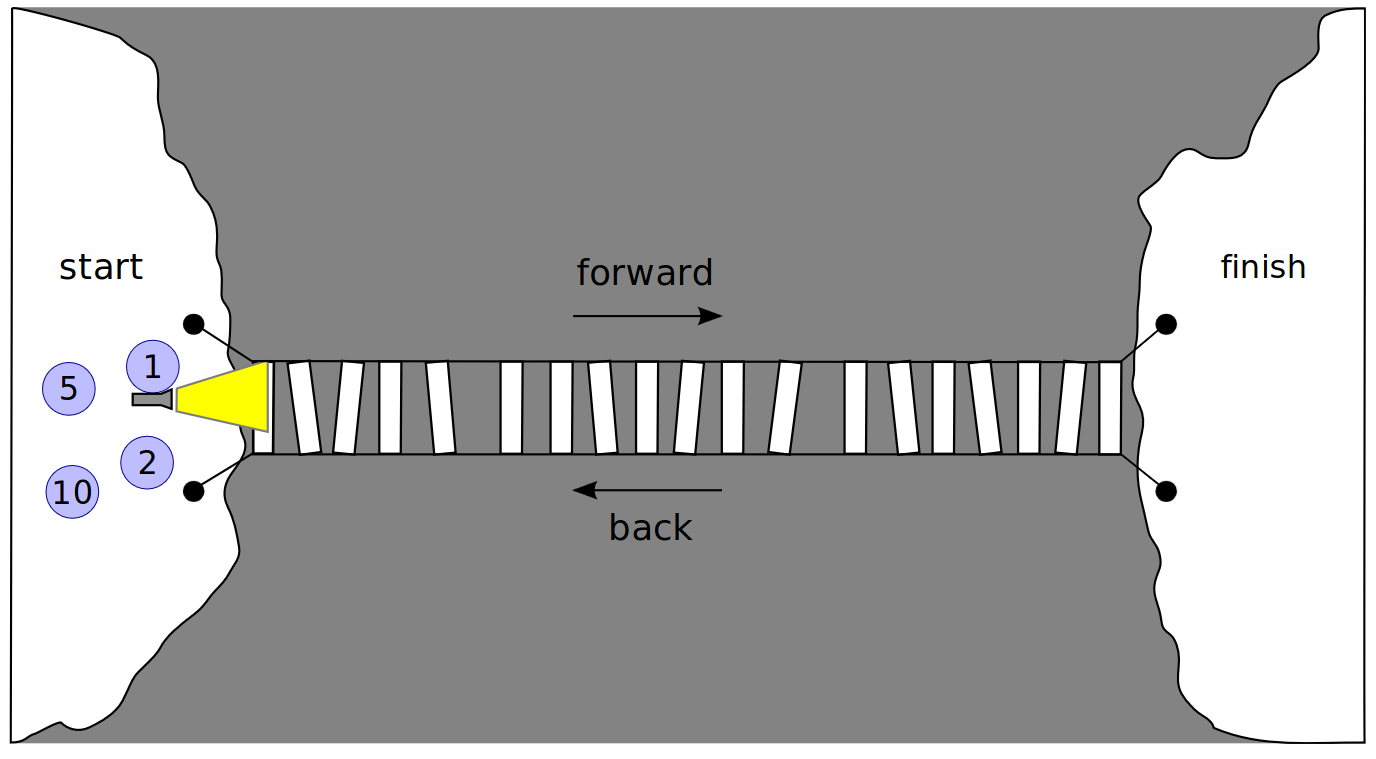
\includegraphics[width=\textwidth]{figures/image.png}
            \caption{Bridge and torch problem}
        \end{figure}
    \end{column}
\end{columns}
\end{frame}

\begin{frame}[fragile]{1st task}

\begin{minted}[
fontsize=\small,
bgcolor=gray!10,
linenos,
breaklines
]{haskell}
changeState :: Objects -> State -> State
changeState o s = \x -> if x == o then not (s o) else s x
\end{minted}

\begin{minted}[
fontsize=\small,
bgcolor=gray!10,
linenos,
breaklines
]{haskell}
getTimeAdv :: Adventure -> Time
getTimeAdv P1 = 1
getTimeAdv P2 = 2
getTimeAdv P5 = 5
getTimeAdv P10 = 10
\end{minted}

\begin{minted}[
fontsize=\small,
bgcolor=gray!10,
linenos,
breaklines
]{haskell}
advsWithLantern :: State -> [Adventurer]
advsWithLantern s = filter (\a -> s (Left a) == s(Right()))
                                            [P1, P2, P5, P10]
\end{minted}

\end{frame}

\begin{frame}[fragile]{1st task}

\begin{minted}[
fontsize=\small,
bgcolor=gray!10,
linenos,
breaklines
]{haskell}
allValidPlays :: State -> ListDur State
allValidPlays s = manyChoice (singles ++ pairs)

      where singles   = [ LD [Duration 
                          (getTimeAdv a,
                          mChangeState [Left a, Right ()] s)]
                        | a <- (advsWithLantern s) ]

            pairs     = [ LD [Duration 
                          (max (getTimeAdv a1) (getTimeAdv a2),
                          mChangeState [Left a1, Left a2, Right ()] s)]
                        | (a1, a2) <- makePairs (advsWithLantern s) ]
\end{minted}

\begin{minted}[
fontsize=\small,
bgcolor=gray!10,
linenos,
breaklines
]{haskell}
data ListDur a = LD [Duration a] deriving Show
manyChoice :: [ListDur a] -> ListDur a
manyChoice = LD . concat . (map remLD)
\end{minted}

\end{frame}

\begin{frame}[fragile]{1st task}

\begin{minted}[
fontsize=\small,
bgcolor=gray!10,
linenos,
breaklines
]{haskell}
exec :: Int -> State -> ListDur State
exec 0 s = return s
exec n s = do s' <- allValidPlays s
              exec (n-1) s'
\end{minted}

\begin{minted}[
fontsize=\small,
bgcolor=gray!10,
linenos,
breaklines
]{haskell}
gFinal :: State
gFinal = const True
\end{minted}

\begin{minted}[
fontsize=\small,
bgcolor=gray!10,
linenos,
breaklines
]{haskell}
leq17 :: Bool
leq17 = any (\(Duration (t,s)) -> s == gFinal && t <= 17)
  (remLD (manyChoice [exec n gInit | n <- [0..5]]))
\end{minted}

It is possible for all adventurers to be on the other side in at most
17 minutes (without exceeding 5 moves) \checkmark
\end{frame}

\begin{frame}[fragile]{1st task}
It is possible for all adventurers to be on the other side in \textbf{less}
than 17 minutes?
\begin{minted}[
fontsize=\small,
bgcolor=gray!10,
linenos,
breaklines
]{haskell}
l17 :: Bool
l17 = any (\(Duration (t,s)) -> s == gFinal && t < 17)
  (remLD (manyChoice [exec n gInit | n <- [0..17]]))
\end{minted}
This takes too long to finish... :(
\begin{minted}[
fontsize=\small,
bgcolor=gray!10,
linenos,
breaklines
]{haskell}
l17 :: Bool
l17 = any (\(Duration (t,s)) -> s == gFinal)
  (remLD (reachableDurStates 17 gInit))
\end{minted}
Solution: BFS (Breadth-First Search).

\end{frame}

\begin{frame}[fragile]{1st task}

\begin{minted}[
fontsize=\small,
bgcolor=gray!10,
linenos,
breaklines
]{haskell}
reachableDurStates :: Int -> State -> ListDur State
reachableDurStates limit s0 = LD (go [Duration (0, s0)] [(s0, 0)])
  where
    go [] _ = []
    go (Duration (t, s) : ws) seen =
      Duration (t, s) : go (ws ++ newNexts) seen'
      where
        nexts = remLD (allValidPlays s)
        newNexts =
          [ Duration (t + dt, s')
          | Duration (dt, s') <- nexts
          , t + dt < limit
          , notElem (s', t + dt) seen
          ]
        seen' =
          map (\(Duration (t', s')) -> (s', t')) newNexts ++ seen
\end{minted}

\end{frame}

\begin{frame}[fragile]{1st task}
It is possible for all adventurers to be on the other side in \textbf{less}
than 17 minutes?
\begin{figure}
            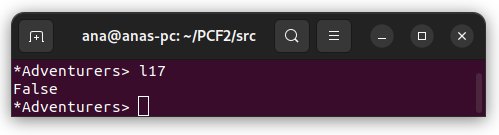
\includegraphics[width=\textwidth]{figures/l17.png}
        \end{figure}
It is \textbf{impossible} for all adventurers to be on the other side in less than 17 minutes!
\end{frame}

\begin{frame}[fragile]{2nd task}

\begin{minted}[
fontsize=\small,
bgcolor=gray!10,
linenos,
breaklines
]{haskell}
probTime :: Int -> Dist Int
probTime x = uniform [x - x `div` 2, x, x + x `div` 2]
\end{minted}

\begin{minted}[
fontsize=\small,
bgcolor=gray!10,
linenos,
breaklines
]{haskell}
play :: Move -> State -> DistDur State
play (Left a) s =
  DD (do t <- probTime (getTimeAdv a)
         return (Duration (t, mChangeState [Left a, Right ()] s)))
play (Right (a1, a2)) s =
  DD (do t1 <- probTime (getTimeAdv a1)
         t2 <- probTime (getTimeAdv a2)
         return (Duration (max t1 t2, mChangeState [Left a1, Left a2, Right ()] s)))
\end{minted}
\end{frame}

\begin{frame}[fragile]{2nd task}
\begin{minted}[
fontsize=\small,
bgcolor=gray!10,
linenos,
breaklines
]{haskell}
instance Ord State where
compare s1 s2 = compare (show s1) (show s2)
\end{minted}

\begin{minted}[
fontsize=\small,
bgcolor=gray!10,
linenos,
breaklines
]{haskell}
plays :: [Move] -> State -> DistDur State 
plays []     s = return s
plays (m:ms) s = do s' <- play m s
                    plays ms s'
\end{minted}
\end{frame}

\begin{frame}[fragile]{2nd task}

\begin{columns}
    \begin{column}{0.4\textwidth}
      \begin{minted}[
fontsize=\small,
bgcolor=gray!10,
linenos,
breaklines
]{haskell}
distExample :: DistDur State
distExample = plays
[Right (P1,P2), Left P1,
Right (P5,P10), Left P2,
Right (P1,P2)] gInit
\end{minted}
"They cannot be all on the other side in less than 19
minutes" \ding{55}
\medskip

"It can be done in 17 minutes" \textbf{\checkmark}

(however, it is not guaranteed, even with optimal moves)
    \end{column}
    \begin{column}{0.6\textwidth}
        \begin{figure}
            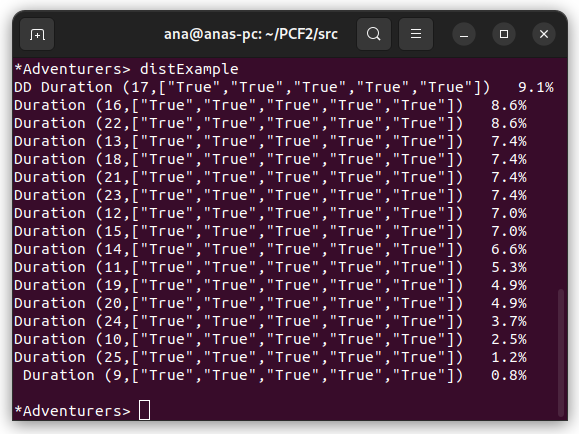
\includegraphics[width=\textwidth]{figures/distExample.png}
        \end{figure}
    \end{column}
\end{columns}
\end{frame}


\begin{frame}[fragile]{3rd task}
      \begin{minted}[
fontsize=\small,
bgcolor=gray!10,
linenos,
breaklines
]{haskell}
game :: IO ()
game = do gameLoop (Duration (0,gInit))
\end{minted}

\begin{minted}[
fontsize=\small,
bgcolor=gray!10,
linenos,
breaklines
]{haskell}
gameLoop :: Duration State -> IO ()
...
\end{minted}

\begin{minted}[
fontsize=\small,
bgcolor=gray!10,
linenos,
breaklines
]{haskell}
applyMove :: Move -> Duration State -> Duration State
...
\end{minted}

\begin{minted}[
fontsize=\small,
bgcolor=gray!10,
linenos,
breaklines
]{haskell}
drawDurationState :: Duration State -> IO ()
...
\end{minted}

\end{frame}

\begin{frame}[fragile]{3rd task}
\begin{figure}
            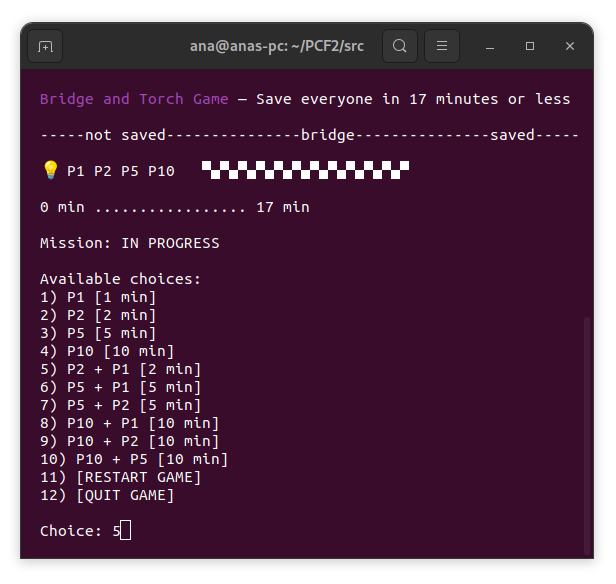
\includegraphics[width=0.55\textwidth]{figures/1.png}
        \end{figure}
\end{frame}

\begin{frame}[fragile]{3rd task}
\begin{figure}
            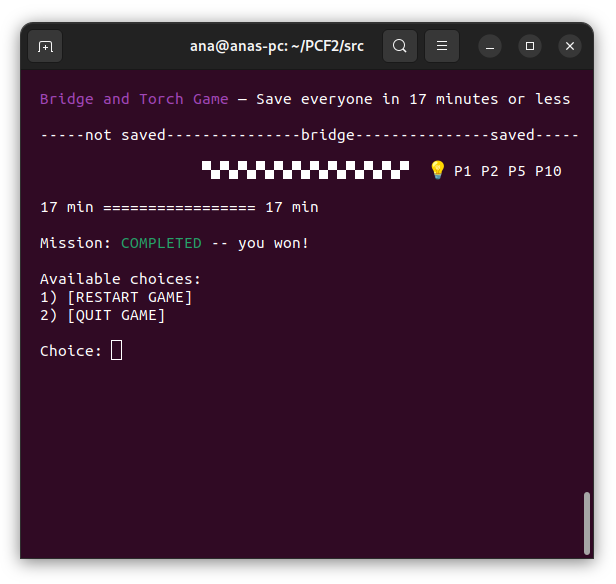
\includegraphics[width=0.55\textwidth]{figures/6.png}
        \end{figure}
\end{frame}

\begin{frame}[fragile]{3rd task}
\begin{figure}
            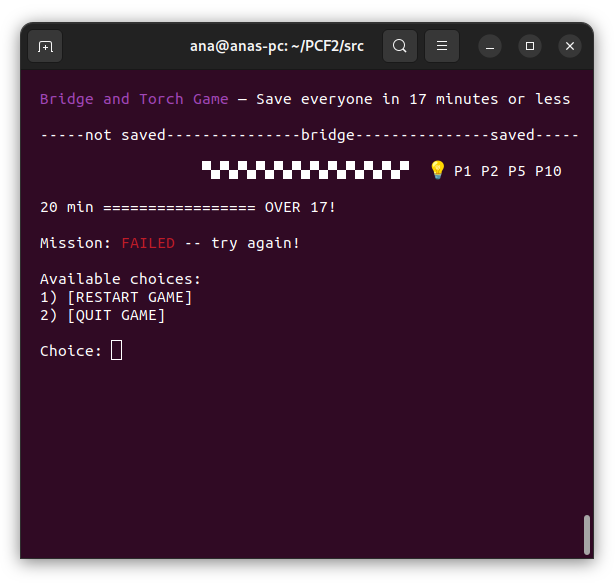
\includegraphics[width=0.55\textwidth]{figures/7.png}
        \end{figure}
\end{frame}

\begin{frame}[fragile]{3rd task}
\begin{minted}[
fontsize=\small,
bgcolor=gray!10,
linenos,
breaklines
]{haskell}
data ListDurLog a = LDL [Duration ([State], a)] deriving Show
...
instance Applicative ListDurLog where
  pure x = LDL [Duration (0, ([], x))]
  ...
instance Monad ListDurLog where
  return = pure
  l >>= k = LDL $ do
    Duration (t, (log1, x)) <- remLDL l
    Duration (t', (log2, y)) <- remLDL (k x)
    return $ Duration (t + t', (log1 ++ log2, y))
\end{minted}
I implemented functions playLog, playsLog, allValidPlaysLog, execLog and more...
\end{frame}

\begin{frame}[fragile]{3rd task}
\begin{minted}[
fontsize=\small,
bgcolor=gray!10,
linenos,
breaklines
]{haskell}
playLog :: Move -> State -> ListDurLog State
playLog (Left a) s =
  LDL [Duration (getTimeAdv a,
  ([mChangeState [Left a, Right ()] s],
  mChangeState [Left a, Right ()] s))]
playLog (Right (a1, a2)) s =
  LDL [Duration (max (getTimeAdv a1) (getTimeAdv a2),
  ([mChangeState [Left a1, Left a2, Right ()] s],
  mChangeState [Left a1, Left a2, Right ()] s))]
\end{minted}

\begin{minted}[
fontsize=\small,
bgcolor=gray!10,
linenos,
breaklines
]{haskell}
playsLog :: [Move] -> State -> ListDurLog State
playsLog []     s = return s
playsLog (m:ms) s = do s' <- playLog m s
                       playsLog ms s'
\end{minted}
\end{frame}

\begin{frame}{3rd task}
\begin{columns}
    \begin{column}{0.5\textwidth}
      showPlaysLog
                \begin{figure}
            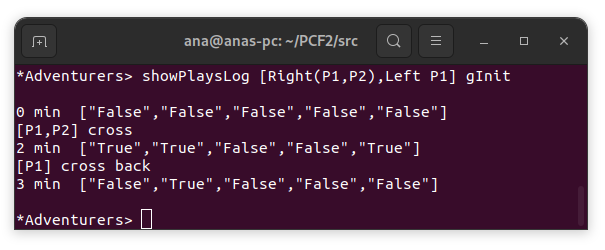
\includegraphics[width=\textwidth]{figures/showPlaysLog.png}
        \end{figure}
    \end{column}
    \begin{column}{0.5\textwidth}
      showPlaysLog2
        \begin{figure}
            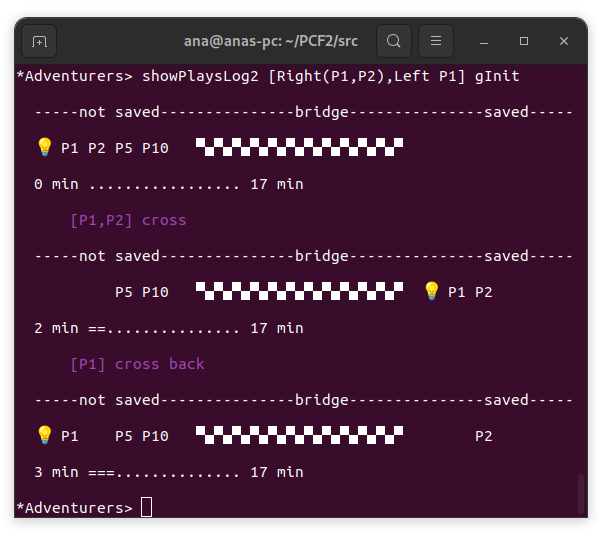
\includegraphics[width=\textwidth]{figures/showPlaysLog2.png}
        \end{figure}
    \end{column}
\end{columns}
\end{frame}

\begin{frame}{3rd task}
\begin{columns}
    \begin{column}{0.5\textwidth}
      printBestPath
                \begin{figure}
            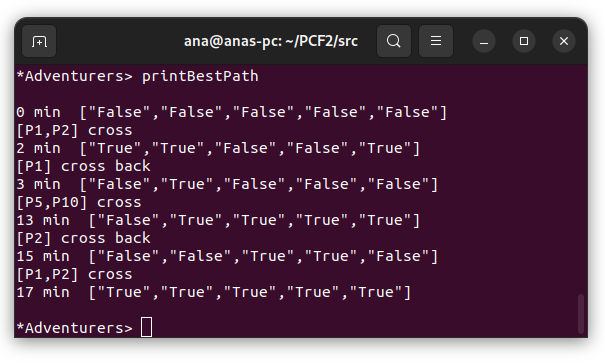
\includegraphics[width=\textwidth]{figures/printBestPath.png}
        \end{figure}
    \end{column}
    \begin{column}{0.5\textwidth}
      printBestPath2
        \begin{figure}
            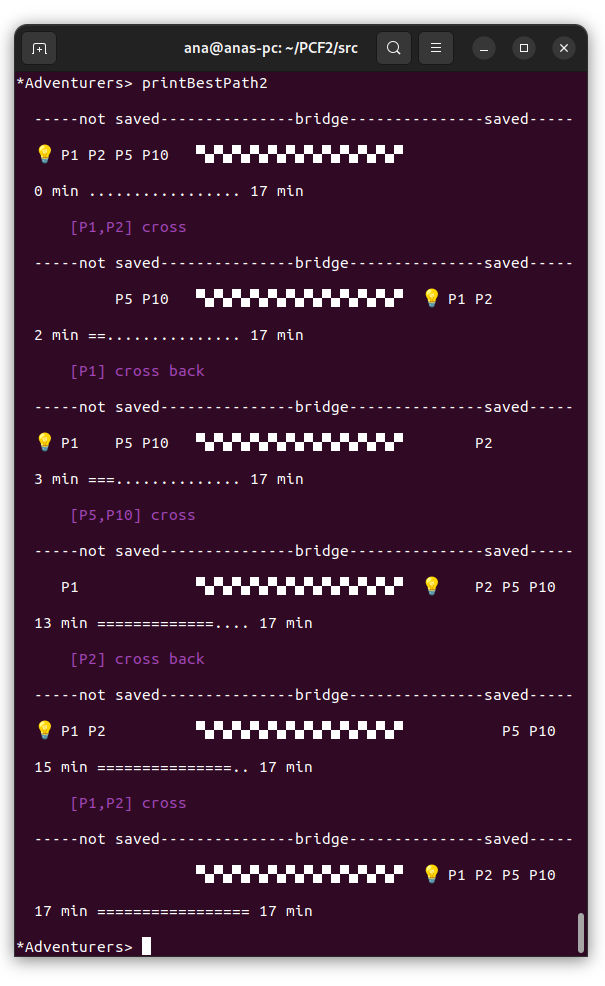
\includegraphics[width=0.4\textwidth]{figures/printBestPath2.png}
        \end{figure}
    \end{column}
\end{columns}
\end{frame}

\begin{frame}{3rd task}
\begin{columns}
    \begin{column}{0.5\textwidth}
                \begin{figure}
            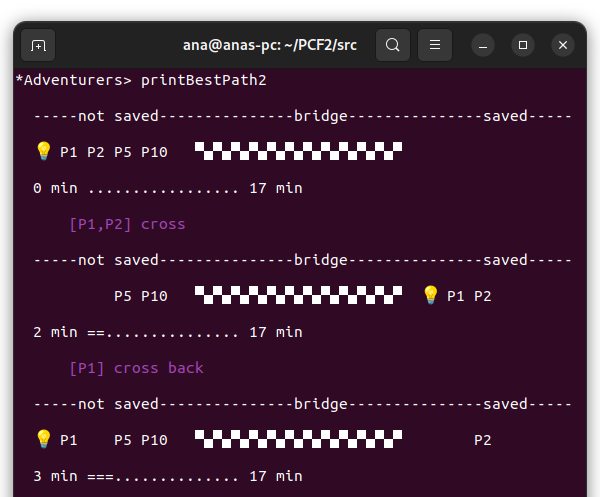
\includegraphics[width=\textwidth]{figures/2.png}
        \end{figure}
    \end{column}
    \begin{column}{0.5\textwidth}
        \begin{figure}
            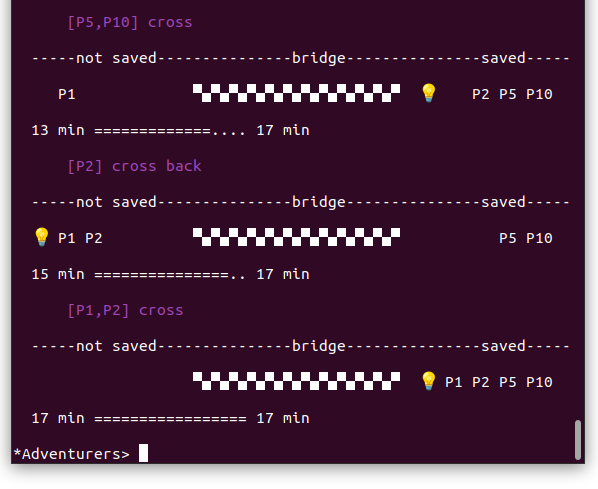
\includegraphics[width=\textwidth]{figures/3.png}
        \end{figure}
    \end{column}
\end{columns}
\end{frame}

\frame{\titlepage}

\end{document}